% Documentación de la Etapa 4
% Compilar con:  pdflatex Informe_etapa4.tex
\documentclass[11pt,a4paper]{article}

\usepackage[utf8]{inputenc}
\usepackage[margin=2.5cm]{geometry}
\usepackage{url}
\usepackage{graphicx}
\usepackage{tikz}

\title{Etapa 4 - AST y Chequeo de Sentencias de MiniJava}
\author{Compiladores e Intérpretes --- UNS, 2026}
\date{}

% Esta instalacion TeX puede no tener las fuentes TS1 (text companion): se evitan
% los simbolos que las requieren (vinetas de itemize, llaves via \{ en \texttt).
\renewcommand{\labelitemi}{$\bullet$}

\begin{document}

\sloppy

\maketitle

\noindent
Implementación de la construcción de los Árboles de Sintaxis Abstracta (AST) de
métodos y constructores y del chequeo de sentencias del analizador semántico de
MiniJava. Se extiende el trabajo de la Etapa 3 (Tabla de Símbolos y chequeo de
declaraciones) para que, durante el parseo, se construya el AST del cuerpo de cada
unidad y, una vez chequeadas y consolidadas las declaraciones, se recorran esos
cuerpos resolviendo nombres, chequeando tipos y validando la información
estructural. No se implementan logros de la etapa; el alcance es el de la
semántica base de sentencias.

\section{Objetivo y logros}

\begin{itemize}
  \item Construir el AST del bloque de cada método y constructor y asociarlo a su
        entrada de la Tabla de Símbolos (TS).
  \item Chequear los cuerpos después del chequeo y la consolidación de
        declaraciones: resolución de nombres, chequeo de tipos, información
        estructural, ámbitos léxicos de variables locales, contexto estático y
        conformidad de tipos de MiniJava.
  \item Reportar el primer error con un mensaje descriptivo y el código
        \texttt{[Error:lexema|nroLinea]}, o \texttt{[SinErrores]} si el programa
        es válido.
\end{itemize}

Se mantienen los logros de etapas anteriores que siguen vigentes (atributos
inicializados, operadores posfijos, visibilidad mejorada, manejo de archivos
eficiente y genericidad avanzada de las Etapas 2 y 3). \textbf{No se intentan
logros de la Etapa 4}: no se implementan MiniLambdas, \texttt{for}, ternario,
\texttt{instanceof}, \texttt{super}, retorno en todos los caminos, floats,
métodos genéricos, multi-detección de errores ni \texttt{main}. La sintaxis
aceptada sigue siendo la de la Etapa 3; los controles agregados son sólo los de
la semántica base de sentencias.

\section{Esquema general}

El módulo principal recibe el archivo fuente, lo asocia al manejador de archivos y
este al léxico. Luego crea la \texttt{TablaDeSimbolos} (que ya carga
\texttt{Object}, \texttt{String} y \texttt{System}) y el
\texttt{AnalizadorSintactico} con dependencia al léxico y a la TS. El sintáctico,
mientras valida la sintaxis, ejecuta las acciones semánticas que insertan las
entidades en la TS, realizan los controles de la primera pasada y construyen el
AST del cuerpo de cada unidad. Al finalizar el parseo, el módulo principal ejecuta
el chequeo de declaraciones (\texttt{estaBienDeclarada}), la consolidación
(\texttt{consolidar}) y, por último, el chequeo de cuerpos
(\texttt{chequearCuerpos}). Si no hay errores informa el mensaje de éxito; ante un
error léxico, sintáctico o semántico captura la excepción correspondiente, reporta
el mensaje y el código de error, y finaliza la ejecución.

\begin{figure}[h]
\centering
\resizebox{\textwidth}{!}{%
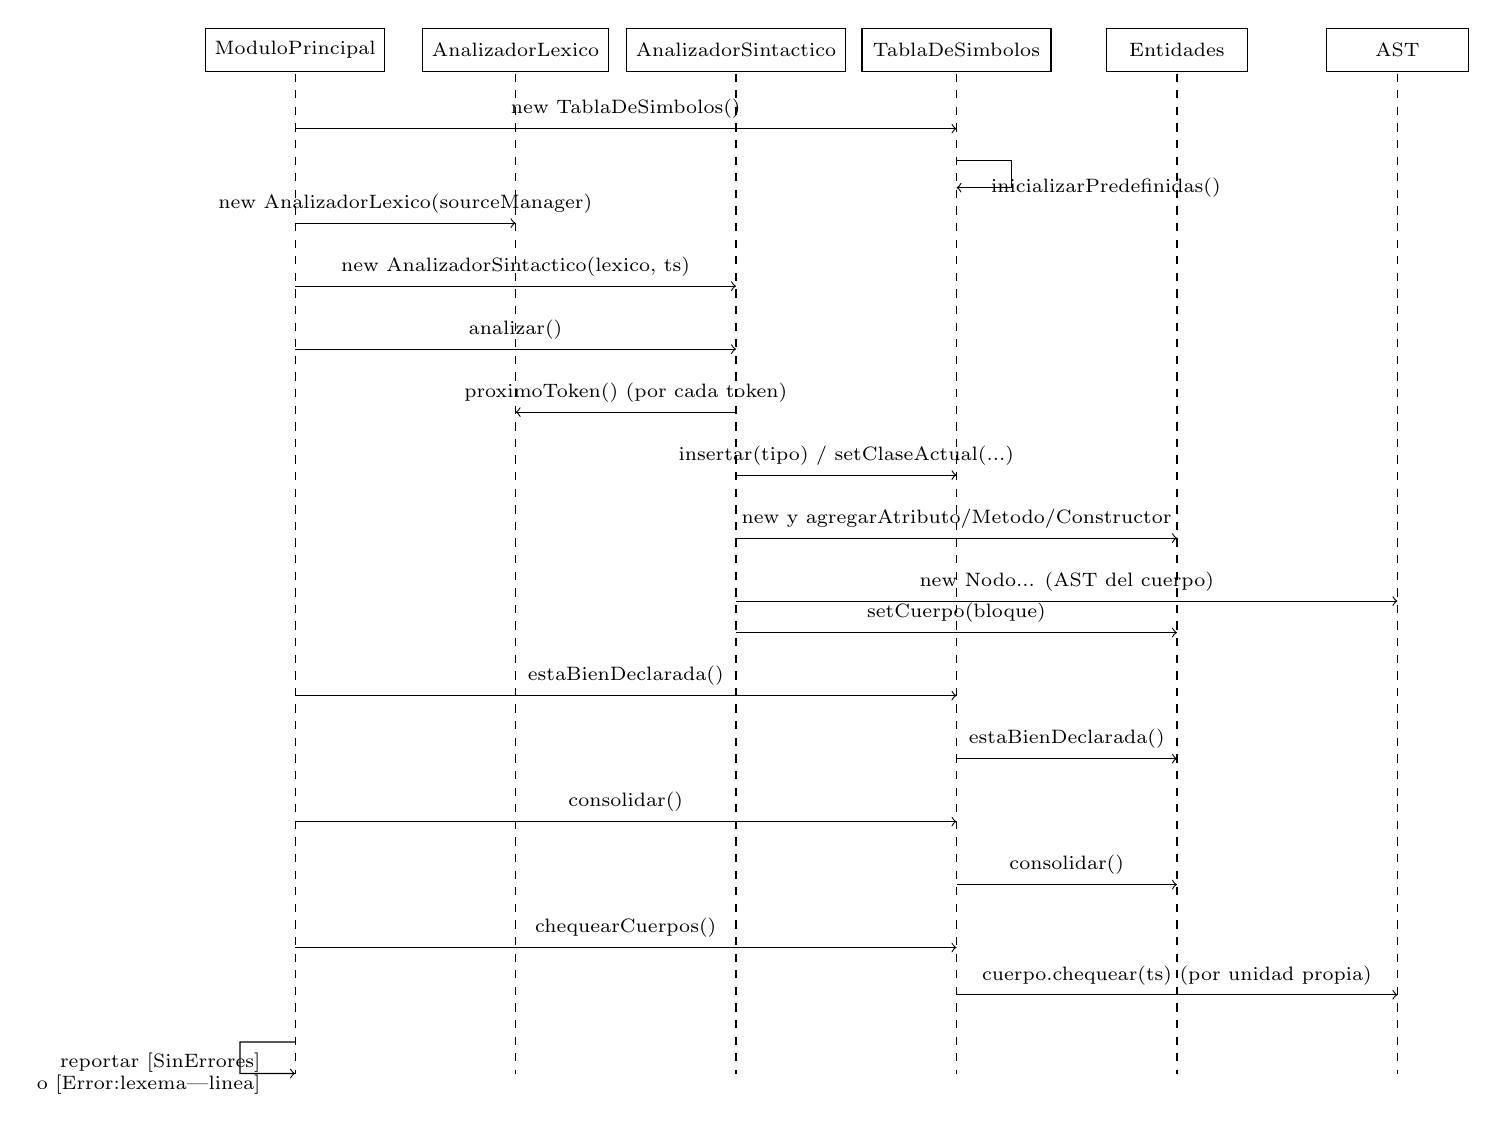
\begin{tikzpicture}[font=\scriptsize]
\def\MP{0}\def\AL{2.8}\def\AS{5.6}\def\TS{8.4}\def\EN{11.2}\def\AST{14.0}
% participantes
\node[draw,minimum width=2.0cm,minimum height=0.55cm] (mp) at (\MP,0) {ModuloPrincipal};
\node[draw,minimum width=2.0cm,minimum height=0.55cm] (al) at (\AL,0) {AnalizadorLexico};
\node[draw,minimum width=2.4cm,minimum height=0.55cm] (as) at (\AS,0) {AnalizadorSintactico};
\node[draw,minimum width=2.4cm,minimum height=0.55cm] (ts) at (\TS,0) {TablaDeSimbolos};
\node[draw,minimum width=1.8cm,minimum height=0.55cm] (en) at (\EN,0) {Entidades};
\node[draw,minimum width=1.8cm,minimum height=0.55cm] (ast) at (\AST,0) {AST};
% lineas de vida
\foreach \x in {\MP,\AL,\AS,\TS,\EN,\AST} { \draw[dashed] (\x,-0.3) -- (\x,-13.0); }
% mensajes
\draw[->] (\MP,-1.0) -- (\TS,-1.0) node[midway,above,align=center]{new TablaDeSimbolos()};
\draw[->] (\TS,-1.4) -- ++(0.7,0) -- ++(0,-0.35) -- (\TS,-1.75)
    node[right,align=left,pos=0.55]{inicializarPredefinidas()};
\draw[->] (\MP,-2.2) -- (\AL,-2.2) node[midway,above,align=center]{new AnalizadorLexico(sourceManager)};
\draw[->] (\MP,-3.0) -- (\AS,-3.0) node[midway,above,align=center]{new AnalizadorSintactico(lexico, ts)};
\draw[->] (\MP,-3.8) -- (\AS,-3.8) node[midway,above,align=center]{analizar()};
\draw[->] (\AS,-4.6) -- (\AL,-4.6) node[midway,above,align=center]{proximoToken() (por cada token)};
\draw[->] (\AS,-5.4) -- (\TS,-5.4) node[midway,above,align=center]{insertar(tipo) / setClaseActual(...)};
\draw[->] (\AS,-6.2) -- (\EN,-6.2) node[midway,above,align=center]{new y agregarAtributo/Metodo/Constructor};
\draw[->] (\AS,-7.0) -- (\AST,-7.0) node[midway,above,align=center]{new Nodo... (AST del cuerpo)};
\draw[->] (\AS,-7.4) -- (\EN,-7.4) node[midway,above,align=center]{setCuerpo(bloque)};
\draw[->] (\MP,-8.2) -- (\TS,-8.2) node[midway,above,align=center]{estaBienDeclarada()};
\draw[->] (\TS,-9.0) -- (\EN,-9.0) node[midway,above,align=center]{estaBienDeclarada()};
\draw[->] (\MP,-9.8) -- (\TS,-9.8) node[midway,above,align=center]{consolidar()};
\draw[->] (\TS,-10.6) -- (\EN,-10.6) node[midway,above,align=center]{consolidar()};
\draw[->] (\MP,-11.4) -- (\TS,-11.4) node[midway,above,align=center]{chequearCuerpos()};
\draw[->] (\TS,-12.0) -- (\AST,-12.0) node[midway,above,align=center]{cuerpo.chequear(ts) (por unidad propia)};
\draw[->] (\MP,-12.6) -- ++(-0.7,0) -- ++(0,-0.4) -- (\MP,-13.0)
    node[left,align=right,pos=0.55]{reportar [SinErrores]\\o [Error:lexema|linea]};
\end{tikzpicture}%
}
\caption{Diagrama de secuencia del análisis de la Etapa 4.}
\end{figure}

\section{Estructura del proyecto}

{\footnotesize
\begin{verbatim}
compilador-minijava/
|-- Compilar.sh / Compilar.bat          Compila y genera Compilador.jar
|-- CorrerTests.sh / CorrerTests.bat    Compila y ejecuta los testers JUnit
|-- lib/                                Jars de JUnit 4 y Hamcrest (se autodescargan)
|-- src/main/java/
|   |-- moduloprincipal/
|   |   \-- ModuloPrincipal.java        Modulo principal (interfaz con el usuario)
|   |-- analizadorlexico/               Etapa 1 (sin cambios)
|   |-- analizadorsintactico/
|   |   |-- AnalizadorSintactico.java   Parser + acciones semanticas (TS y AST)
|   |   \-- ExcepcionSintactica.java    Error sintactico
|   |-- analizadorsemantico/            Tabla de Simbolos y chequeos
|   |   |-- TablaDeSimbolos.java        Tabla global, predefinidas, ambitos, cuerpos
|   |   |-- Entidad.java                Entidad declarable (abstracta)
|   |   |-- Unidad.java                 Metodo/Constructor (abstracta)
|   |   |-- Clase.java / Interfaz.java  Tipos declarados
|   |   |-- Metodo.java / Constructor.java / Atributo.java / Parametro.java
|   |   |-- VariableLocal.java / Bloque.java
|   |   |-- Tipo.java y subclases       Modelo de tipos (primitivo, void, T, arreglo, ref)
|   |   |-- InfoCheck.java              Tipo + asignable + llamada
|   |   |-- SemanticaUtil.java          Conformidad, vistas genericas, contexto
|   |   \-- ExcepcionSemantica.java     Error semantico
|   |-- analizadorsemantico/ast/        NUEVO: nodos del AST (expresiones y sentencias)
|   \-- sourcemanager/                  Etapa 1 (sin cambios)
|-- src/test/java/test/                 Testers JUnit provistos por la catedra
\-- resources/
    |-- sinErrores/                     Casos de prueba sin errores
    \-- conErrores/                     Casos de prueba con errores
\end{verbatim}
}

\section{Diseño e implementación de los AST}

Cada tipo de nodo es una clase; la herencia modela las relaciones ``es-un''. Los
nodos conservan tokens para poder reportar el error con el lexema y la línea
correctos.

\subsection{Gramática de diseño y gramática de construcción}

Los tipos de nodo del AST se \emph{diseñan} a partir de la gramática original del
lenguaje (los constructores sintácticos que tienen significado), pero el AST se
\emph{construye} durante el análisis sintáctico con una Especificación Dirigida
por la Traducción (EDT) sobre la gramática LL(1) que efectivamente implementa el
parser. La cátedra pide explícitamente esta separación: el diseño se guía por la
gramática original, mientras que la construcción se hace sobre la gramática del
parser.

Las diferencias entre ambas gramáticas se resuelven en el parser, no en el diseño:

\begin{itemize}
  \item \textbf{Recursión a izquierda}: \texttt{ExpresionCompuesta} y
        \texttt{Referencia} son recursivas a izquierda en la gramática original.
        La versión LL(1) (\texttt{ECResto}, \texttt{RResto}) las reconoce con
        recursión a derecha y las arma con un acumulador, produciendo árboles
        asociativos a izquierda.
  \item \textbf{Sentencias de expresión}: la gramática original distingue
        \texttt{Sentencia ::= Asignacion ;} y \texttt{Sentencia ::= Llamada ;},
        pero ambas son alias de \texttt{Expresion}. La transformación LL(1) las
        unifica en \texttt{Sentencia ::= Expresion ;}; por eso hay un único
        \texttt{NodoSentenciaExpresion}, que clasifica la forma durante el
        chequeo (\texttt{NodoExpresionAsignacion} vs. \texttt{InfoCheck.esLlamada()}).
\end{itemize}

Correspondencia entre producciones de la gramática original y nodos del AST:

{\footnotesize
\begin{verbatim}
Produccion (gramatica original)              Nodo
------------------------------------------   --------------------------
AccesoVar ::= idMetVar                       NodoVar
LlamadaMetodo ::= idMetVar ArgsActuales      NodoLlamada
LlamadaMetodoEstatico                        NodoLlamadaEstatica
LlamadaConstructor ::= new TipoRef Args      NodoNewObjeto
CrearArreglo ::= new TipoBase Dimensiones    NodoNewArreglo
ExpresionParentizada                         NodoExpresionParentizada
Primario this / stringLiteral                NodoThis / NodoLiteral
Primitivo                                    NodoLiteral
Expresion con OperadorAsignacion             NodoExpresionAsignacion
ExpresionCompuesta con OperadorBinario       NodoExpresionBinaria
ExpresionBasica con OperadorUnario           NodoExpresionUnaria
PosfijoOpcional (solo en la LL(1))           NodoExpresionPosfijo
VarEncadenada ::= . idMetVar                 NodoEncadenadoAtributo
MetodoEncadenado ::= . idMetVar Args         NodoEncadenadoLlamada
AccesoArreglo ::= [ Expresion ]              NodoEncadenadoArreglo
Bloque / Sentencia ;                         NodoBloque / NodoSentenciaVacia
VarLocal / Return / If / While               NodoVarLocal / NodoReturn / NodoIf / NodoWhile
Sentencia ::= Asignacion ; / Llamada ;       NodoSentenciaExpresion
\end{verbatim}
}

En síntesis: los \textbf{tipos de nodo} reflejan los constructores significativos
de la gramática original; la \textbf{forma del árbol} es la que produce el parseo
LL(1) implementado.

\subsection{Jerarquía de expresiones}

{\footnotesize
\begin{verbatim}
NodoExpresion (abstracta)
|-- NodoLiteral
|-- NodoThis
|-- NodoVar
|-- NodoLlamada
|-- NodoLlamadaEstatica
|-- NodoNewObjeto
|-- NodoNewArreglo
|-- NodoExpresionParentizada
|-- NodoExpresionBinaria
|-- NodoExpresionUnaria
|-- NodoExpresionPosfijo
|-- NodoExpresionAsignacion
\-- NodoReferencia --------------------+
                                        | usa
NodoEncadenado (abstracta) <-----------+
|-- NodoEncadenadoAtributo
|-- NodoEncadenadoLlamada
\-- NodoEncadenadoArreglo
\end{verbatim}
}

\texttt{NodoReferencia} modela \texttt{Primario RResto}: un primario seguido de un
encadenado opcional. Cada eslabón recibe el tipo estático del receptor, lo controla
y delega en el siguiente. Esto cubre accesos como \texttt{crearPersona().edad},
\texttt{matriz[0].length} o \texttt{caja.obtener().toString()}.

\subsection{Jerarquía de sentencias}

{\footnotesize
\begin{verbatim}
NodoSentencia (abstracta)
|-- NodoBloque
|-- NodoSentenciaVacia
|-- NodoSentenciaExpresion
|-- NodoVarLocal
|-- NodoReturn
|-- NodoIf
\-- NodoWhile
\end{verbatim}
}

\subsection{Diagrama de clases}

{\footnotesize
\begin{verbatim}
                       +----------------------------+
                       |       NodoExpresion        |
                       |       <<abstracta>>        |
                       +----------------------------+
                       | # token: Token             |
                       +----------------------------+
                       | + chequear(ts): InfoCheck  |
                       | + getTokenValor(): Token   |
                       | + getTokenSentencia():Token|
                       +-------------+--------------+
                                     |
   +--------+--------+--------+-----+-----+--------+--------+--------+
   |        |        |        |           |        |        |        |
   v        v        v        v           v        v        v        v
 Nodo     Nodo    Nodo     Nodo        Nodo     Nodo     Nodo     Nodo
 Literal  This    Var      Llamada     Llamada  New      New      Expresion
                           /           Estatica Objeto   Arreglo  Parentizada
                           | args                                    |
                           v                                         v
                      NodoExpresion                          NodoExpresion
   (ademas: NodoExpresionBinaria, NodoExpresionUnaria, NodoExpresionPosfijo,
            NodoExpresionAsignacion, NodoReferencia)

                       +----------------------------+
                       |       NodoReferencia       |
                       +----------------------------+
                       | - primario: NodoExpresion  |
                       | - encadenado: NodoEncadenado (0..1)
                       +-------------+--------------+
                                     | usa
                                     v
                       +----------------------------+
                       |       NodoEncadenado       |
                       |       <<abstracta>>        |
                       +----------------------------+
                       | # token: Token             |
                       | # siguiente: NodoEncadenado|
                       +----------------------------+
                       | + chequear(ts, receptor)   |
                       +-------------+--------------+
                                     |
                    +----------------+----------------+
                    v                v                 v
            NodoEncadenado   NodoEncadenado    NodoEncadenado
              Atributo          Llamada           Arreglo

                       +----------------------------+
                       |       NodoSentencia        |
                       |       <<abstracta>>        |
                       +----------------------------+
                       | # token: Token             |
                       +----------------------------+
                       | + chequear(ts): void       |
                       +-------------+--------------+
                                     |
   +---------+---------+-------------+-----------+---------+---------+
   |         |         |             |           |         |         |
   v         v         v             v           v         v         v
 Nodo      Nodo      Nodo          Nodo        Nodo      Nodo      Nodo
 Bloque    Sentencia Sentencia     VarLocal    Return    If        While
           Vacia     Expresion
\end{verbatim}
}

\subsection{Métodos de chequeo}

\begin{itemize}
  \item Toda expresión implementa \texttt{InfoCheck chequear(TablaDeSimbolos ts)}.
  \item Toda sentencia implementa \texttt{void chequear(TablaDeSimbolos ts)}.
  \item Toda expresión aplica el patrón de \textbf{responsabilidad + delegación}:
        controla lo propio y delega en sus hijos.
  \item Cada expresión expone además \texttt{getTokenValor()} (token que la
        representa en contextos que exigen un tipo: condición, retorno, argumento)
        y \texttt{getTokenSentencia()} (token señalado cuando no es admisible como
        sentencia).
\end{itemize}

\section{Construcción de los AST durante el análisis sintáctico}

Se modificó \texttt{AnalizadorSintactico} para que las acciones semánticas
construyan nodos, siguiendo una EDT sobre la gramática LL(1) que el parser ya
implementaba. Los tipos de nodo provienen del diseño guiado por la gramática
original; la traducción de las reglas recursivas a izquierda se hace con
acumuladores en el parser.

\subsection{Sentencias}

{\footnotesize
\begin{verbatim}
Produccion                                   Nodo construido
------------------------------------------   --------------------------
Bloque                                       NodoBloque
Sentencia ;                                  NodoSentenciaVacia
Expresion ;                                  NodoSentenciaExpresion
var id = ExpresionCompuesta                  NodoVarLocal
return ExpresionOpcional                     NodoReturn
if (Expresion) Sentencia else Sentencia      NodoIf
while (Expresion) Sentencia                  NodoWhile
\end{verbatim}
}

\subsection{Expresiones}

\begin{itemize}
  \item \texttt{expresion()} construye \texttt{NodoExpresionAsignacion} si
        aparece \texttt{=}.
  \item \texttt{expresionCompuesta()} / \texttt{eCResto()} construyen
        \texttt{NodoExpresionBinaria} asociando a izquierda, respetando el único
        nivel de binarios de la gramática.
  \item \texttt{expresionBasica()} construye \texttt{NodoExpresionUnaria} y
        \texttt{NodoExpresionPosfijo}.
  \item \texttt{referencia()} construye \texttt{NodoReferencia} cuando hay
        encadenado y devuelve el primario directo cuando no lo hay.
  \item \texttt{rResto()} encadena \texttt{NodoEncadenadoAtributo},
        \texttt{NodoEncadenadoLlamada} y \texttt{NodoEncadenadoArreglo}.
  \item \texttt{primario()} construye \texttt{NodoThis}, \texttt{NodoLiteral}
        (string), \texttt{NodoVar}, \texttt{NodoLlamada}, \texttt{NodoNewObjeto},
        \texttt{NodoNewArreglo}, \texttt{NodoLlamadaEstatica} o
        \texttt{NodoExpresionParentizada}.
\end{itemize}

\subsection{Asociación a la TS}

Al terminar de parsear el bloque de un método o constructor, el nodo se asocia a
la unidad antes de insertarla en la clase:

{\footnotesize
\begin{verbatim}
NodoBloque cuerpo = bloque();
Metodo metodo = new Metodo(tokenNombre, tipoRetorno, parametros, esEstatico, ts);
metodo.setCuerpo(cuerpo);
agregarMetodo(metodo);
\end{verbatim}
}

\section{Chequeo de sentencias}

El chequeo se ejecuta \textbf{después} de \texttt{estaBienDeclarada()} y
\texttt{consolidar()}. \texttt{TablaDeSimbolos.chequearCuerpos()} recorre las
clases y, para cada una, sólo las unidades propias; así un cuerpo heredado no se
rechequea en el descendiente.

\subsection{Resolución de nombres}

Para un identificador sin receptor (\texttt{NodoVar}) se busca en este orden:

\begin{enumerate}
  \item variable local visible (bloque actual hacia contenedores),
  \item parámetro de la unidad actual,
  \item atributo de la clase actual (incluidos los heredados consolidados).
\end{enumerate}

Si se selecciona un atributo en contexto estático se reporta error. Si no se
encuentra, ``la variable X no fue declarada''.

Para llamadas implícitas (\texttt{NodoLlamada}) se busca la clave
\texttt{(nombre, aridad)} en los métodos de la clase actual, incluidos los
heredados. En contexto estático sólo se admiten métodos estáticos.

Para receptores explícitos se usa el \textbf{tipo estático} del receptor:

\begin{itemize}
  \item referencias: se busca el miembro en la clase/interfaz y se aplica la
        sustitución genérica correspondiente a la vista;
  \item interfaces: además de sus propios métodos, ofrecen los métodos de
        instancia de \texttt{Object} (por ejemplo \texttt{toString}), pero no sus
        métodos estáticos ni los de la clase que las implementa;
  \item arreglos: sólo \texttt{length} (sólo lectura) y \texttt{toString()} sin
        argumentos;
  \item primitivas, \texttt{null}, \texttt{void} o parámetros de tipo no
        instanciados no permiten seleccionar miembros.
\end{itemize}

\subsection{Chequeo de tipos}

\begin{itemize}
  \item Operadores: \texttt{int} para \texttt{+ - * / \%} y comparaciones;
        \texttt{boolean} para \texttt{\&\& || !}; \texttt{== !=} exigen
        conformidad en alguna dirección; sin promociones ni concatenación con
        \texttt{+}.
  \item Asignación: el lado izquierdo debe ser asignable y el derecho debe
        conformar con el izquierdo. El resultado tiene el tipo del destino y no es
        asignable.
  \item Llamadas y creaciones: se controla aridad y que cada argumento conforme
        con el formal correspondiente.
  \item Creación de arreglos: cada dimensión debe ser \texttt{int}; el tipo base
        debe ser válido y, si es genérico, no puede omitirse el argumento.
  \item \texttt{var}: el inicializador se chequea antes de declarar la variable;
        no se admite \texttt{void} ni \texttt{null} como origen de inferencia.
  \item \texttt{if} / \texttt{while}: la condición debe ser \texttt{boolean}.
  \item \texttt{return}: en \texttt{void} sólo \texttt{return;}; en métodos con
        retorno, \texttt{return e;} con conformidad; en constructores sólo
        \texttt{return;}.
\end{itemize}

\subsection{Información estructural}

\texttt{InfoCheck} porta \texttt{asignable} y \texttt{llamada}. Reglas
implementadas:

\begin{itemize}
  \item locales, parámetros, atributos, componentes de arreglo: asignables;
  \item \texttt{length}: no asignable;
  \item literales, \texttt{this}, paréntesis, resultados de operadores,
        asignaciones, creaciones: no asignables;
  \item una llamada a método o la creación de un objeto son admisibles como
        sentencia de llamada; una creación de arreglo no lo es;
  \item una expresión parentizada conserva el tipo pero \textbf{pierde} ambas
        propiedades (\texttt{(x) = 3}, \texttt{(x = 3);}, \texttt{(metodo());},
        \texttt{(objeto).metodo();} se rechazan);
  \item una sentencia de expresión sólo es válida si es una asignación o termina
        en una llamada (por eso \texttt{crearPersona().edad;} se rechaza aunque su
        tipo sea asignable).
\end{itemize}

\subsection{Ámbitos y declaraciones locales}

\begin{itemize}
  \item Al entrar a un bloque se crea un ámbito; al salir se restaura el anterior.
  \item Una local no puede repetir el nombre de un parámetro de la unidad ni el de
        una local visible en el bloque actual o en un contenedor.
  \item Puede ocultar un atributo.
  \item Bloques hermanos pueden reutilizar nombres.
  \item El inicializador no ve a la variable que se está declarando.
  \item Se rechaza una declaración local como cuerpo directo de \texttt{if},
        \texttt{else} o \texttt{while}.
  \item Se chequean todas las sentencias, incluso después de un \texttt{return}
        (no se rechaza código inalcanzable).
\end{itemize}

\subsection{Contexto estático}

\begin{itemize}
  \item No se permite \texttt{this} ni el acceso implícito a atributos o métodos
        de instancia.
  \item Sí se permite acceder a miembros de instancia mediante un receptor
        explícito obtenido de un parámetro, local, llamada o creación.
  \item Se rechaza el parámetro de tipo de la clase en encabezados y cuerpos de
        métodos estáticos (incluido dentro de arreglos o argumentos genéricos).
\end{itemize}

\subsection{Conformidad de MiniJava}

Se respetaron explícitamente las diferencias con Java:

\begin{itemize}
  \item genéricos y arreglos invariantes;
  \item sin tipos raw (fuera de la excepción de herencia sin argumento);
  \item sin cotas para parámetros de tipo;
  \item herencia genérica sin argumento conserva el parámetro original; un
        parámetro conservado se identifica por su declaración de origen, de modo
        que dos parámetros que comparten letra pero provienen de declaraciones
        distintas no conforman entre sí;
  \item arreglos conforman con \texttt{Object}, pero no entre arreglos de distinto
        tipo base;
  \item \texttt{null} conforma con referencias, parámetros y arreglos, no con
        primitivas;
  \item \texttt{void} no conforma con tipos de valor.
\end{itemize}

\section{Entidades predefinidas}

Antes de analizar el programa la tabla contiene:

\begin{itemize}
  \item \texttt{Object}, que declara \texttt{String toString()} (de instancia) y
        \texttt{static void debugPrint(int)}; tiene un constructor por defecto;
  \item \texttt{String}, tipo de los literales de cadena, que hereda de
        \texttt{Object}, tiene constructor por defecto y no declara métodos
        propios;
  \item \texttt{System}, que hereda de \texttt{Object} y declara los métodos
        estáticos \texttt{read()}, \texttt{printB(boolean)}, \texttt{printC(char)},
        \texttt{printI(int)}, \texttt{printS(String)}, \texttt{println()},
        \texttt{printBln(boolean)}, \texttt{printCln(char)}, \texttt{printIln(int)}
        y \texttt{printSln(String)}.
\end{itemize}

Toda clase sin relación explícita extiende \texttt{Object} y hereda sus miembros;
una clase que implementa una interfaz también es un subtipo de \texttt{Object}.
Los arreglos ofrecen únicamente \texttt{length} y el \texttt{toString()} de
\texttt{Object}. Una interfaz no puede declarar un método con la misma clave que
un método de instancia de \texttt{Object} con signatura distinta.

\section{Reporte de errores}

Al detectarse un error se reporta y finaliza la ejecución. El token asociado sigue
las pautas de la cátedra: se señala el token del nodo que tiene el error. En
particular:

\begin{itemize}
  \item errores de creación: la palabra reservada \texttt{new};
  \item errores de selección de miembro o de indexación: el selector \texttt{.} o
        el corchete \texttt{[};
  \item errores de tipo de un índice, tamaño, retorno o condición: la
        subexpresión ofensora (por ejemplo el índice, el tamaño o el valor
        retornado);
  \item llamadas implícitas no resueltas: el nombre del método;
  \item argumentos de una llamada con receptor explícito: el nombre del método;
  \item asignaciones y operadores: el operador correspondiente.
\end{itemize}

{\footnotesize
\begin{verbatim}
Error Semantico en linea <N>: <mensaje>
[Error:<lexema>|<N>]
\end{verbatim}
}

\section{Formato de salida}

\subsection{Análisis exitoso}

{\footnotesize
\begin{verbatim}
Compilacion Exitosa
[SinErrores]
\end{verbatim}
}

\subsection{Análisis con errores}

Mensaje descriptivo seguido del código de error, por ejemplo:

{\footnotesize
\begin{verbatim}
Error Semantico en linea 5: el tipo boolean no conforma con el tipo de retorno int
[Error:true|5]
\end{verbatim}
}

\section{Compilación y ejecución}

No se usa ninguna herramienta de build: solo se necesitan \texttt{javac},
\texttt{jar} y \texttt{java} de cualquier JDK 21 o superior (probado con JDK 25).

{\footnotesize
\begin{verbatim}
./Compilar.sh             # compila y genera Compilador.jar  (Windows: Compilar.bat)
java -jar Compilador.jar resources/sinErrores/semIICorrecto01.java
./CorrerTests.sh          # compila y ejecuta los testers JUnit  (Windows: CorrerTests.bat)
\end{verbatim}
}

\subsection{Comandos manuales equivalentes}

Compilar (desde \texttt{compilador-minijava/}):

{\footnotesize
\begin{verbatim}
javac -d build/classes \
  src/main/java/moduloprincipal/*.java \
  src/main/java/analizadorlexico/*.java \
  src/main/java/analizadorsintactico/*.java \
  src/main/java/analizadorsemantico/*.java \
  src/main/java/analizadorsemantico/ast/*.java \
  src/main/java/sourcemanager/*.java
jar cfe Compilador.jar moduloprincipal.ModuloPrincipal -C build/classes .
\end{verbatim}
}

Correr los tests (desde \texttt{compilador-minijava/}, con JUnit 4.13.2 y Hamcrest
1.3 en \texttt{lib/}):

{\footnotesize
\begin{verbatim}
javac -cp "build/classes:lib/junit-4.13.2.jar:lib/hamcrest-core-1.3.jar" \
  -d build/test-classes src/test/java/test/*.java

java -cp "build/classes:build/test-classes:lib/junit-4.13.2.jar:\
lib/hamcrest-core-1.3.jar" org.junit.runner.JUnitCore \
  test.TesterDeCasosSinErrores test.TesterDeCasosConErrores
\end{verbatim}
}

En Windows el separador del classpath es \texttt{;} en lugar de \texttt{:}.

\section{Tests}

Se incluyen los casos provistos por la cátedra y casos propios desarrollados para
esta etapa (el diseño de los casos de prueba es responsabilidad del alumno).
Resultado actual: \textbf{404/404 casos OK}.

Los testers descubren automáticamente todos los archivos de
\texttt{resources/sinErrores/} y \texttt{resources/conErrores/}. La batería
utilizada es la de la cátedra (archivos \texttt{TAMBIENBORRAR\_*.txt}) junto con
los casos base \texttt{semIIError*.java} y \texttt{semIICorrecto*.java}. Los
archivos antiguos de convención previa que contradecían a la batería nueva se
apartaron en \texttt{tests\_descartados/} para que los testers no los descubran.

Los casos sin errores cubren, entre otros: predefinidas y uso de
\texttt{Object.debugPrint} y \texttt{toString} (en clases, interfaces, arreglos y
cadenas); creación de \texttt{Object} y \texttt{String}; herencia encadenada;
redefinición exacta; sobrecarga por aridad; implementación de interfaces (simples,
con extensión y genéricas); clases genéricas con parámetros en atributos, retornos
y parámetros; herencia genérica con y sin argumento; vistas genéricas en accesos y
llamadas; arreglos multidimensionales; \texttt{this}, \texttt{length},
\texttt{if}, \texttt{while}, \texttt{null}; métodos estáticos; paréntesis y
pérdida de propiedades estructurales; y declaraciones locales con visibilidad por
bloques.

Los casos con errores cubren, entre otros: nombres de tipo repetidos;
redeclaración de las predefinidas; relaciones de herencia inválidas o circulares;
atributos y métodos repetidos; redefiniciones con firma distinta; contratos de
interfaces; tipos inválidos; argumentos genéricos inválidos (incluidos anidados);
tipos raw; operadores y asignaciones con tipos incompatibles; resolución de
nombres y ámbitos; contexto estático; información estructural de sentencias
(asignabilidad y forma de llamada); indexación y creación de arreglos; y retornos
inválidos.

\section{Fuera de alcance (logros)}

No se implementaron los logros de la etapa: MiniLambdas, \texttt{for}, retorno en
todos los caminos sin código muerto, floats y coerción, ternario, genericidad
avanzada (inferencia por diamante completa), \texttt{instanceof}, visibilidad,
\texttt{super}, métodos genéricos, multi-detección de errores, atributos
inicializados, postfijos como sentencia ni \texttt{main}. La sintaxis aceptada
sigue siendo la de la Etapa 3; los controles agregados son sólo los de la
semántica base de sentencias.

\section{Anexo A - Diferencias de sintaxis respecto de la gramática original}

El parser implementado (heredado de las Etapas 2 y 3) acepta algunos constructos
que no figuran en el archivo de la gramática original ni en la semántica base. Se
listan para dejar explícita la diferencia; el chequeo de sentencias de la Etapa 4
base no los trata de forma especial.

{\footnotesize
\begin{verbatim}
Constructo                    Gramatica original   Gramatica implementada (LL1)
---------------------------   ------------------   ----------------------------
public / private              no figuran           VisibilidadOpcional
Posfijos ++ / --              no figuran           PosfijoOpcional
Argumentos genericos anidados no                   instanciadoOParametrico recursivo
Notacion diamante new Caja<>  no                   admitida si la clase es generica
\end{verbatim}
}

Estas extensiones provienen de los logros de las Etapas 2 y 3. Los controles
semánticos de esta entrega que las alcanzan son los mínimos: por ejemplo, el
posfijo se admite sólo dentro de expresiones y sobre operandos \texttt{int}
asignables, y \texttt{new Caja<>()} no infiere el argumento (eso corresponde al
logro de genericidad avanzada).

\end{document}
